\chapter{Architecture of Chord}
\label{chap:architecture}

Figure \ref{fig:architecture} depicts the architecture of Chord.  The following sections explain each component of Chord in more detail.

\begin{figure}
\begin{center}
\begin{label}{fig:architecture}
%\texonly{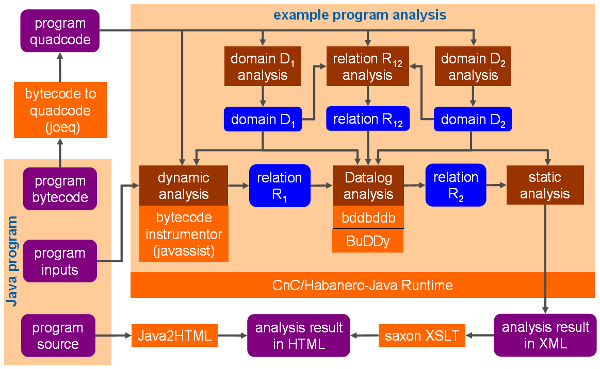
\includegraphics[scale=0.7]{chord_arch.png}}
\htmlonly{{\htmlimg{chord_arch.png}}}
\caption{Architecture of Chord}
\end{label}
\end{center}
\end{figure}

{\bf Under Construction}

%\section{Inputs}
%The inputs to Chord are:
%\begin{itemize}
%\item
%Various system properties dictating the desired configuration and functionality of Chord.
%Chapter \ref{chap:properties} describes how to set properties and the meaning of properties
%recognized by Chord.
%\item
%A Java program to be analyzed.  The program is specified in terms of the main class of the program (via property \code{chord.main.class}) and the application classpath of the program (via property \code{chord.class.path}).  These two properties suffice if only static analysis will be performed; if dynamic analysis is desired, then command-line arguments to run the program must also be provided (via property \code{chord.args}).  Chord analyzes Java bytecode, not source code; however, if it is desired to present analysis results at the Java source level, then the Java source path of the program must also be provided (via property \code{chord.src.path}).
%\end{itemize}
%
%\section{Chord Project}
%project: classic or modern
%analyses determined by ...
%\section{Program Analyses}
%dynamic analysis: \ref{chap:dynamic-analysis}
%Datalog analysis: \ref{chap:datalog-analysis}
%\section{Outputs}

